
%(BEGIN_QUESTION)
% Copyright 2012, Tony R. Kuphaldt, released under the Creative Commons Attribution License (v 1.0)
% This means you may do almost anything with this work of mine, so long as you give me proper credit

The ``flare'' at an oil refinery functions as a safe way to quickly dispose of pressurized hydrocarbon compounds, by burning them far away from anything else that might be flammable.  In this system, as with most flare systems, a ``knockout drum'' exists to separate vapors from liquid, so that only vapors are sent to the flare tip to be burned.  Any captured liquid is drained to the Oily Water Sewer (OWS) system:

$$\includegraphics[width=15.5cm]{i0002rx01.eps}$$

As with most flare systems, the exact composition of material sent to the flare to be burned is both highly variable and unknown from moment to moment.  In a typical refinery, anything from hydrogen gas to diesel fuel might get sent to the flare during a ``depressurization'' event.

\vskip 10pt

Suppose operations personnel at this refinery wish to monitor the total flow rate of hydrocarbon material burned at the flare.  Engineers are debating what type(s) of flowmeter might be used for this task, and where exactly it should be placed in the piping system.

\vskip 10pt

Brainstorm some different flow-sensing technologies, and then determine whether or not each one of them could be applied to this problem.

\underbar{file i00977}
%(END_QUESTION)





%(BEGIN_ANSWER)

First, the proper location of the vapor flowmeter: between the knockout drum and the water-seal drum, or between the water-seal drum and the flare tip.  Proper straight-pipe lengths should be observed in order to achieve best measurement accuracy.

\vskip 10pt

\begin{itemize}
\item{} {\bf Orifice plate/venturi/etc.} -- Probably not suitable, due to the unknown density ($\rho$) of the vapors going through the pipe.  If a gas density analyzer were added to the system, and its signal used along with absolute pressure and temperature compensation, accurate measurement of either volumetric or mass flow might be possible.
\vskip 10pt
\item{} {\bf Positive displacement} -- Probably not suitable, due to possible particulate matter in the gas stream, and rapid temperature changes.  Most importantly, if this flowmeter ever jammed, it would ``plug up'' the flare and prevent its safe operation!
\vskip 10pt
\item{} {\bf Turbine} -- Possibly suitable.  Pressure and temperature compensation would both be necessary to calculate true volumetric flow rate, however.
\vskip 10pt
\item{} {\bf Vortex} -- Probably not suitable, due to low-flow cutoff interfering with operation at low flare flow rates.  Even if minimum flow could be ensured, pressure and temperature compensation would both be necessary to calculate true volumetric flow rate.
\vskip 10pt
\item{} {\bf Magnetic} -- Definitely unsuitable, due to non-conductivity of vapors in general.
\vskip 10pt
\item{} {\bf Ultrasonic} (Doppler) -- Definitely unsuitable, due to lack of objects in flow stream to reflect sound waves. 
\vskip 10pt
\item{} {\bf Ultrasonic} (transit time) -- Possibly suitable.  Pressure and temperature compensation would both be necessary to calculate true volumetric flow rate, however.
\vskip 10pt
\item{} {\bf Coriolis} -- Definitely suitable, but most likely too expensive to consider for this application.
\vskip 10pt
\item{} {\bf Thermal mass} -- Definitely unsuitable, due to the unknown and randomly changing specific heat of flare vapors.
\end{itemize}

 
%(END_ANSWER)





%(BEGIN_NOTES)


%INDEX% Process: flare knockout drum and water seal (realistic P&ID shown)

%(END_NOTES)


